\documentclass[fullpage]{article}
	\addtolength{\oddsidemargin}{-.875in}
	\addtolength{\evensidemargin}{-.875in}
	\addtolength{\textwidth}{1.75in}

	\addtolength{\topmargin}{-.875in}
	\addtolength{\textheight}{1.75in}

\makeatletter
\setlength{\@fptop}{0pt}
\makeatother
\usepackage[utf8]{inputenc}
\usepackage[pdftex]{graphicx}
\usepackage{mathtools}
\usepackage{float}
\usepackage{amsfonts}
\usepackage{subcaption}


\title{\textbf{Computational Robotics} \\  Lab 1 - Markov Decision Processes}
\author{Name: Andrew Choi, UID: 205348339}
\date{October 2019}

\begin{document}
\maketitle

\section{Introduction}

The goal of this lab is to explore Markov Decision Processes to control a simple discretized robot in a discrete finite state space environment for which a perfect model is provided. To do so, a gridworld is constructed with well-defined transition probabilities and rewards. In this gridworld, a model for the robot's behavior is developed and implemented to accomplish a prescribed task by constructing optimal policies through dynamic programming. This lab report first describes the mathematical foundation necessary to understand the contents of the report along with the experimental setup and results.

\section{Mathematical Formulation}

\subsection{Markov Decision Processes}
Before delving into the details of the experiment, the Markov Decision Process as well as the methods employed to solve it (value iteration and policy iteration) are described briefly mathematically.

Markov decision processes (abbreviated MDP from hereon) are a classical formalization of discrete time sequential decision making. Driven by rewards, actions are made by an agent not just influenced by immediate rewards gained by a certain action, but also by a discounted sum of possible future rewards. Therefore, the MDP allows an agent to make decisions that take into consideration both future consequences and opportunities. Figure 1 from Sutton and Barto's \textit{Reinforcement Learning} shows this agent environment relation. The MDP can be described as a tuple
\[
(S, A, P, R, H, \gamma),
\]
where $S$ is the finite state space, $A$ is the finite action space, $P$ is the transition probabilities between states given a certain action, $R$ is the immediate reward received from transitioning to a certain state, $H$ is the horizon, and $\gamma$ is the discount factor. The transition probabilities for an MDP are the probabilities of transitioning to all possible next states given a current state and action as shown below. They model an environment's stochasticity and are a necessary component for dynamic programming methods.
\[
\sum_{s' \in S} P_{sa}(s') = 1 \; \forall s \in S
\]
Provided these parameters, MDPs provide solutions to problems that satisfy the Markov property which states that all the information that is needed to make a decision at the current time step is the current state $s$ and action $a$. With a problem framed as an MDP that satisfies the Markov property, the goal is then to find an optimal policy $\pi^*(s)$ that outputs the optimal action for every state in the state space. To find such a policy, the value function is introduced in the next section as well as its role and relation in deriving the optimal policy.  

\begin{figure}[H]
\centering
\includegraphics[width=50mm]{images/agent_env_relation.jpg}
\caption{The agent-environment interaction in a Markov decision process.}
\label{fig:gridworld}
\end{figure}

\subsection{Value Functions and Policies}
The value function $V^\pi(s) \; \forall s \in S$, is the expected sum of discounted returns for every state under a given policy. By taking into account all future rewards, the value function provides a metric for determining which states are favorable and lead to high rewards and which should be avoided. Furthermore, the discount factor $\gamma$ can be tuned to vary the weight given to future rewards versus immediate rewards.
\[
V^\pi = \mathbb{E}[\sum_t^\infty \gamma^t r(s_t)]
\]
The value function is different depending on the policy $\pi(s)$ that is followed which deterministically chooses an action depending on the current state. For any MDP, there exists one unique optimal value function $V^*(s)$. From this optimal value function, an optimal policy $\pi^*(s)$ can be derived. Although there exists only one unique optimal value function, there may exist multiple optimal policies arising from multiple actions resulting in tie values.
To derive the optimal value function for finite state spaces we use two dynamic programming methods, policy iteration and value iteration. These two methods both employ the Bellman operator iteratively in their own distinct ways. Although the methodology of these two methods are different they both achieve the same result of computing an optimal policy. First, policy iteration is discussed.

\subsection{Policy Iteration}
The first step of policy iteration is to randomly initialize a policy $\pi_0$. Afterwards, a two step loop is started until an optimal policy is reached. This loop consists of

\begin{enumerate}
\item Policy Evaluation $\rightarrow$ Computing $V^\pi$ for the current policy
\item Policy Improvement $\rightarrow$ Leveraging knowledge gained from $V^\pi(s)$ to improve the policy
\end{enumerate}

Policy evaluation consists of its own iterative loop in which the value function for a policy is continuously updated until convergence using the Bellman operator where the previous value function estimate is used to obtain a better value function estimate. Each loop step can be thought of as extending the time horizon starting from 0 towards $H$ which effectively propagates the discounted rewards throughout the states.
\begin{gather}
V^{\pi_{t+1}} = \mathbb{E}_{s'}[r(s, a, s') + \gamma V^{\pi_t}(s')] \\
V^{\pi_{t+1}} = \sum_{s'} P_{sa}(s') [r(s, a, s') + \gamma V^{\pi_t}(s')]
\end{gather}
Policy evaluation ends when the policy does not change which occurs when the value function has converged to its true value. This convergence can be defined by a certain threshold as shown below.
\begin{gather}
\lVert V^{\pi_{t+1}} - V^{\pi_{t}} \lVert \; < threshold 
\end{gather}
Once a value function for a policy is computed, policy improvement can then be undergone to create a new improved policy. This is done by analyzing the value function of the previous policy and seeing where differents actions for certain states could have led to higher expected discounted returns. The policy is then changed accordingly.
\begin{gather}
\pi_{t+1} = argmax_a V^{\pi_i}(s)
\end{gather}
Using this new policy, policy evaluation is undergone once more and the loop continues. This iterative loop ends when the policy no longer changes due to convergence to the optimal value function which in turn leads to the optimal policy.
\begin{gather}
V^* = V^{\pi_{t+1}} \\
\pi^* = \pi_{t+1} = argmax_a \mathbb{E}_{s'}[r(s, a, s') + \gamma V^*(s')]
\end{gather}

\subsection{Value Iteration}
In contrast to policy iteration, value iteration never explicity deals with a policy. Instead the Bellman operator is applied to an initialized value function iteratively until the value function converges to the optimal value function. Rather than computing value functions for certain policies and improving upon those policies, value iteration can be thought of as updating the value function for every single possible action in every state. Due to this, only once the optimal value function is found is then a policy generated. It should be evident that such a policy would be an optimal policy. Below are the steps of value iteration. 

\begin{gather}
\text{initialize} \; V_0^*(s) = 0 \; \forall s \in S \\
\text{loop step 10} \\
V^*(s) = {max}_a \mathbb{E}_{s'}[r(s, a, s')] = {max}_a \sum_{s'} P_{sa}(s') r(s, a, s') \\
V_{t+1}^*(s) = {max}_a \sum_{s'} P_{sa}(s') [r(s, a, s') + \gamma V_t^*(s')] \\
\text{stop when} \; \lVert V_{t+1} - V_t \lVert \; < threshold \\
V^*(s) = V_{t+1}(s) \\
\pi^*(s) = argmax_a V^*(s)
\end{gather}


\section{Experimental Setup}

\subsection{Robot Description}

For the experiment, a simple robot is considered that will reside in the gridworld and attempt to reach a prescribed goal state. The robot will occupy one grid in the gridworld at any given time and can face any of the twelve headings identified by the hours on a clock $h \in \{0...11\}$. Each action is characterized by a movement value of 1, -1, or 0 which can be thought of as moving forward, backward, or staying still, respectively. This movement is then followed by a rotation of 1, -1, 0 which can be thought of as clockwise, counter-clockwise, and no rotation. Following this, it can be seen that the action of the robot can be described as a tuple
\[
(a, b),
\]
where $a$ is the movement value and $b$ is the rotation value. The following restrictions are also applied to the robot's actions:
\begin{enumerate}
\item Attempting to move off the grid results in no linear movement, but the rotation portion will still happen.
\item Aside from restriction 1, the robot can only rotate if it also moves forwards or backwards.
\item If the robot chooses to move, a pre-rotation error may occur with probability $p_e$
\begin{enumerate}
\item With probability $p_e$ each, the robot will first rotate by +1 or -1 before it moves. No pre-rotate with probability $1-2*p_e$.
\item Choosing to stay still will not incur an error rotation.
\end{enumerate}
\item The robot will move one unit in the direction it is facing, rounded to the nearest cardinal direction.
\end{enumerate}
Then, it can be seen that the robot has the following discrete action space and size.
\[
(1, 0), (1, 1), (1,-1), (0,0), (-1,0), (-1,1), (-1,1), \; \; N_e = 7
\]
The discrete state space is the set of all possible (x, y) positions and heading angles and can be described by tuple
\[
(x, y, h)
\]
where $x \in \{0...7\}$ is the x position on the grid, $y \in \{0...7\}$ is the y position on the grid, and $h \in \{0...11\}$ is the heading angle of the robot. Following this, the state space size can be computed as
\[
N_s = X*Y*R = 8*8*12 = 768
\]

\subsection{Created Gridworld and Rewards}
To simulate the MDP system, an 8x8 gridworld is constructed through software. Provided are the rewards for the states of the gridworld as shown in figure 2 where boundary states (red and marked X) have reward -100, lane markers (yellow and marked -) have reward -10, and the goal state (green and marked *) has reward +1. All other states have reward 0.

\begin{figure}[t!]
\centering
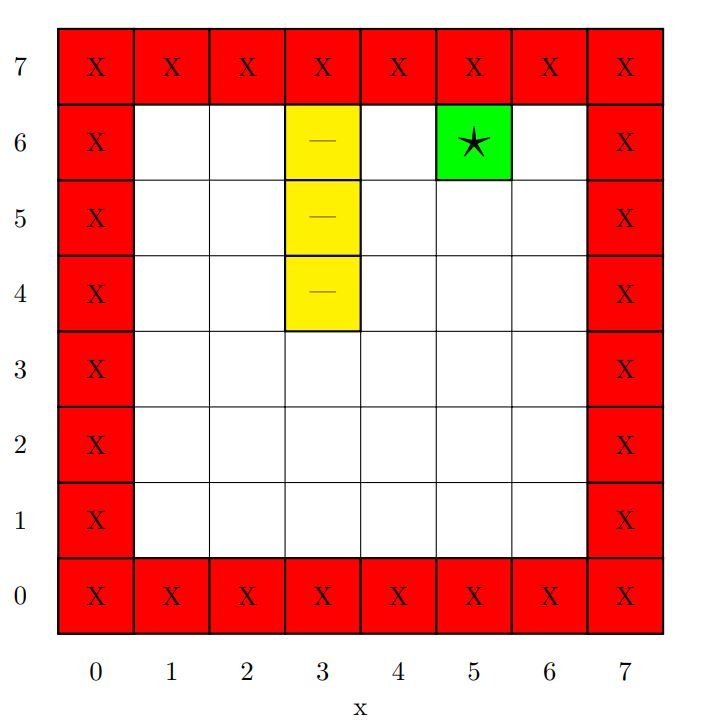
\includegraphics[width=60mm]{images/gridworld.jpg}
\caption{Gridworld with Rewards}
\label{fig:gridworld}
\end{figure}

\subsection{Benchmark}
To be able to properly analyze the effects of following an optimal policy, a benchmark must first be set. This benchmark will be the trajectory generated by a hand-engineered initial policy $\pi_0$. This policy crudely gets to the goal state by prioritizing closing the x distance and then the y distance without any regard for rewards \textit{(code in utils.py)}.

\subsection{Scenarios}
With the following setup, four different scenarios are explored:
\begin{enumerate}
\item Reward at goal state located at (x=5, y=6) independent of heading, $p_e = 0\%$
\item Reward at goal state located at (x=5, y=6) independent of heading, $p_e=25\%$
\item Scenario 1 but reward of +1 only when robot is pointing down $h=6$
\item Scenario 2 but reward of +1 only when robot is pointing down $h=6$
\end{enumerate}
All four scenarios start out at an initial state of $(x=1, y=6, h=6)$ with a discount factor of $\gamma = 0.9$. Code has been generated that can graphically plot and generate trajectories according to the different parameters above. In the next section, the results of such trajectories as well as any computational differences between value and policy iteration are analyzed and discussed.

\section{Experimental Results}

\subsection{Scenario 1}

\begin{figure}[H]
\begin{subfigure}{.5\textwidth}
\centering
\includegraphics[width=75mm]{images/pe0_ip.jpeg}
\caption{Initial Policy Trajectory}
\label{fig:a}
\end{subfigure}
\begin{subfigure}{.5\textwidth}
\centering
\includegraphics[width=75mm]{images/pe0_pi.jpeg}
\caption{Policy Iteration Trajectory}
\label{fig:b}
\end{subfigure}
\begin{subfigure}{.5\textwidth}
\centering
\includegraphics[width=75mm]{images/pe0_vi.jpeg}
\caption{Value Iteration Trajectory}
\label{fig:c}
\end{subfigure}
\caption{Scenario 1 Trajectory Results}
\end{figure}

Generated trajectories for the initial policy and value/policy iteration can be seen above in figure 3 for when $p_e = 0\%$ and the goal state is independent of robot heading. With $p_e$ equaling zero, this effectively eliminates any stochasticity in the environment. Therefore, the above trajectories will remain unchanged if generated again since actions deterministically get the robot to the state it desires. In subfigure (a), it can be seen that the initial policy does well avoiding any negative reward positions but takes an unnecessarily wide turn around the lane markers resulting in a total reward of +1 over 14 time steps to reach the goal. In contrast, both value iteration and policy iteration, result in a total reward of +1 while only taking 10 time steps to reach the goal by optimizing to take the tightest possible turn around the lane markers. In fact, the trajectories for both methods are identical. Although they are identical, it should be noted that each method may come up with different optimal policies as discussed earlier in section 2.2.
To compare computational differences, the runtimes for both methods to convergence were measured with Python's time library over ten separate runs and averaged with the results being as follow.
\[
PI_{time} = 6.201 \; seconds \; \; VI_{time} = 6.323 \; seconds
\]
With a difference of only about a tenths of a second, there seems to be no noticeable difference in terms of computational speed between the two methods for scenario 1. This is to be expected as the state space is at a manageable size and actions are deterministic leading to a relatively easy optimization problem compared to the other scenarios.

\subsection{Scenario 2}

For scenario 2, stochasticity is now introduced into the environment by setting $p_e$ to 25\%. This stochasticity is rather large as the robot will not experience a random rotation with a 50\% probability. Unlike scenario 1, different runs will now result in different trajectories due to sampling from a distribution of possible next states. Therefore, two plots each for the initial policy, policy iteration, and value iteration are included as shown in figure 4 to have a more comprehensive representation of possible trajectories. Furthermore, the results of the six shown trajectories are summarized below in table 1.
\begin{table}[H]
\centering
\begin{tabular}{lll}
\hline
Trajectory & Total Reward & Number of Time Steps to Goal \\ \hline
IP Traj 1 & -19          & 18                           \\
IP Traj 2 & -1099           & 30                            \\
PI Traj 1 & +1           & 32                           \\
PI Traj 2 & +1           & 14                           \\
VI Traj 1 & +1           & 18                           \\
VI Traj 2 & +1           & 18                          
\end{tabular}
\caption{Scenario 2 Trajectory Results}
\end{table}

At first glance, one commonality between the trajectories is that they often have accidental detours and must turn completely around or even end up in cyclical paths due to random chance rotations. Unique to the initial policy, is that it often arrives at states with negative reward during its trajectories. Trajectory 4(a) is somewhat successful but ends up moving across two of the lane markers leading to a negative total reward of -19. On the other hand, trajectory 4(b) experiences an exceptionally bad trajectory that ends up with a total reward of -1099. It can be seen that after running into the red border states, it gets stuck moving back and forth along the edge for a total of 11 time steps until it finally breaks out.

In contrast, both value iteration and policy iteration successfully avoid negative reward states regardless of any unfavorable states encountered. This is done even if it ends up increasing the time it takes to the goal as shown in trajectory 4(c) in particular. Since we have not assigned a penalty regarding number of actions taken, the policies produced by both methods dictate the robot's actions in a way that maximizes the probability of success even if it means extending the time horizon. This explains the cyclical path shown in trajectory 4(c). It should be understood that differences in trajectory between policy iteration and value iteration are arbitrary and are due to chance. Overall, it can be seen that regardless of which method is used, both produce robust policies that maximizes the probability of success of achieving a task in the face of uncertainty. Compared to scenario 1, a noticeable difference in computational time is now observed as shown below.
\[
PI_{time} = 10.492 \; seconds \; \; VI_{time} = 6.664 \; seconds
\]
Policy iteration starts to take about 4 seconds longer to converge. Value iteration on the other hand increases by only about three tenths of a second. This may be due to introducing stochasticity into the environment which may lead to a harder optimization problem requiring additional runs of policy iteration.

\begin{figure}[H]
\begin{subfigure}{.5\textwidth}
\centering
\includegraphics[width=70mm]{images/pe25_ip.jpeg}
\caption{Initial Policy Trajectory 1}
\label{fig:1a}
\end{subfigure}
\begin{subfigure}{.5\textwidth}
\centering
\includegraphics[width=70mm]{images/pe25_ip_s4.jpeg}
\caption{Initial Policy Trajectory 2}
\label{fig:1b}
\end{subfigure}
\begin{subfigure}{.5\textwidth}
\centering
\includegraphics[width=70mm]{images/pe25_pi.jpeg}
\caption{Policy Iteration Trajectory 1}
\label{fig:2a}
\end{subfigure}
\begin{subfigure}{.5\textwidth}
\centering
\includegraphics[width=70mm]{images/pe25_pi2.jpeg}
\caption{Policy Iteration Trajectory 2}
\label{fig:2b}
\end{subfigure}
\begin{subfigure}{.5\textwidth}
\centering
\includegraphics[width=70mm]{images/pe25_vi.jpeg}
\caption{Value Iteration Trajectory 1}
\label{fig:3a}
\end{subfigure}
\begin{subfigure}{.5\textwidth}
\centering
\includegraphics[width=70mm]{images/pe25_vi2.jpeg}
\caption{Value Iteration Trajectory 2}
\label{fig:3b}
\end{subfigure}
\caption{Scenario 2 Trajectory Results}
\end{figure}


\subsection{Scenario 3}

Scenario 3 explores a deterministic setting once again by setting $p_e$ back to 0. For this scenario, the goal state now only occurs when the robot is facing down at the (x=5, y=6) position. Rather than comparing to the initial policy's trajectory as a benchmark, it may be better to compare the trajectories produced by value and policy iteration to those in scenario 1 in order to see what effect narrowing the goal state has had on the trajectory. The trajectories for scenario 3 are shown below in figure 5. After inspection, it is observed that both scenarios regardless of method output exactly the same path aside from the robot's heading. In scenario 1, since the goal state was independent of the robot's heading angle, the robot arbitrarily moved "forwards" while facing up. In contrast, due to the goal state requiring the robot to be in the $h=6$ heading position, the robot takes advantage of its ability to move backwards to align itself in correct orientation without sacrificing time efficiency in scenario 3. Whereas before in scenario 1 where the robot had multiple optimal policies to choose from, scenario 3 leads to a more narrow set of optimal policies. Much like before, computational times are computed as the average of 10 runs.
\[
PI_{time} = 10.048 \; seconds \; \; VI_{time} = 7.016 \; seconds
\]
Similar to scenario 2, policy iteration suffers from longer convergence times compared to value iteration. Surprisingly, this happens even without any stochasticity in the environment. 

\begin{figure}[H]
\begin{subfigure}{.5\textwidth}
\centering
\includegraphics[width=75mm]{images/pe0_pi_s3.jpeg}
\caption{Policy Iteration Trajectory}
\label{fig:a}
\end{subfigure}
\begin{subfigure}{.5\textwidth}
\centering
\includegraphics[width=75mm]{images/pe0_vi_s3.jpg}
\caption{Value Iteration Trajectory}
\label{fig:b}
\end{subfigure}
\caption{Scenario 3 Trajectory Results}
\end{figure}

\subsection{Scenario 4}

Quite easily the most difficult task for the robot to achieve, scenario 4 reintroduces stochasticity into the environment while also narrowing the set of goal states. Much like scenario 2, two trajectories are shown each for value and policy iteration to get a better representation of trajectory possibilities. Furthermore, results of both methods are compared to those in scenario 2 and are summarized in table 2.

\begin{table}[H]
\centering
\begin{tabular}{lll}
\hline
Trajectory & Total Reward & Number of Time Steps to Goal \\ \hline
PI Traj 1  & +1           & 42                           \\
PI Traj 2  & +1           & 12                           \\
VI Traj 1  & +1           & 26                           \\
VI Traj 2  & +1           & 14                          
\end{tabular}
\caption{Scenario 4 Trajectory Results}
\end{table}

Very similar to scenario 2, it can be observed that both methods once again produce robust policies that avoid any encounter with undesired states. Despite the uncertainty of the system, the robot is still able to successfully arrive at the goal state even with the restriction of having to face pointing down. In trajectory 6(a), the robot actually arrives at the goal state in time step 38 but has to leave the goal state due to an unwanted rotation occuring and reenter the goal state concluding its trajectory at time step 42. Trajectory 6(c) shows an instance of several cyclical paths which further shows the robot's willingness to take additional actions in exchange for a higher probability of maximizing its total sum of discounted rewards. Once again, there is no real difference in the results when using policy or value iteration. Both methods achieve the same result of producing robust optimal policies but differ in convergence speed.
\[
PI_{time} = 11.263 \; seconds \; \; VI_{time} = 7.480 \; seconds
\]
The convergence times for both methods have increased which aligns with the difficulty of the scenario's task. Similar to scenarios 2 and 3, value iteration once again converges faster by about four seconds. It is often difficult to pinpoint exactly why such a difference occurs as there are several factors dependent on the problem setting that go into determining the convergence speeds of both methods. It can be concluded with high confidence that at least for this MDP system, with the current initial state and prescribed tasks, value iteration is more efficient.

\begin{figure}[H]
\begin{subfigure}{.5\textwidth}
\centering
\includegraphics[width=70mm]{images/pe25_pi_s4.jpeg}
\caption{Policy Iteration Trajectory 1}
\label{fig:2a}
\end{subfigure}
\begin{subfigure}{.5\textwidth}
\centering
\includegraphics[width=70mm]{images/pe25_pi2_s4.png}
\caption{Policy Iteration Trajectory 2}
\label{fig:2b}
\end{subfigure}
\begin{subfigure}{.5\textwidth}
\centering
\includegraphics[width=70mm]{images/pe25_vi_s4.jpeg}
\caption{Value Iteration Trajectory 1}
\label{fig:3a}
\end{subfigure}
\begin{subfigure}{.5\textwidth}
\centering
\includegraphics[width=70mm]{images/pe25_vi2_s4.png}
\caption{Value Iteration Trajectory 2}
\label{fig:3b}
\end{subfigure}
\caption{Scenario 4 Trajectory Results}
\end{figure}

\section{Conclusion}
In this lab, a robot planning problem on a 2D grid was solved. This was done by framing the problem as a Markov decision process. With access to the environment's transition probabilities as well as the state space being computationally finite, dynamic programming methods, value and policy iteration, were used to compute optimal policies for the robot under several scenarios. This was made possible by using a value function which contained the expected sum of discounted rewards for every state allowing for future consequences and opportunities to be considered during decision making. 

Regardless of the scenario, both methods produced robust optimal policies that led to the robot successfully reaching the goal state without encountering any negative reward states. This was especially evident when comparing trajectories produced by a crudely hand-engineered initial policy which continuously ran into unfavorable states when the environment became stochastic. Even with the further restriction of narrowing the goal state to require a specific heading, both methods once again succeeded in producing policies that avoided negative reward states. It was shown that there was no difference in results between the two methods as they both arrive at the same optimal value function. The one thing that did differ between the methods was the computational speed in which value iteration converged faster by about 40\% in three out of four scenarios.

Lastly, although dynamic programming methods can be effective in computing optimal policies, their requirement of having access to the transition probabilities as well as operating over a finite state space limits their applicability to most real world robotics problems in which the transition probabilities are either inaccurate or unknown. Furthermore, with many high level robotics problems occuring in a continuous state space, dynamic programming methods would be computationally infeasable. Regardless of this fact, given the right circumstances, both value and policy iteration result in producing optimal control policies for a problem framed as a Markov decision process.

\section{Sources}

Sutton, R. S. and A. G. Barto. 2017. Reinforcement Learning: An Introduction (2nd Edition). MIT Press.


\end{document}